% !TEX root =  main.tex

\subsection{Repeated Nesting}
\label{sec:exp-repeat-app}

We next consider some simple models with multiple levels of nesting, starting with
\begin{subequations}
	\label{eq:repeat-nest}
\begin{align}
y^{(0)} \sim \mathrm{Uniform}(0,1), \quad &
y^{(1)} \sim \mathcal{N}(0,1), \quad
y^{(2)} \sim \mathcal{N}(0,1), \displaybreak[0] \\ 
f_0 \left(y^{(0)}, \gamma_1\left(y^{(0)}\right)\right)&= \log \gamma_1\left(y^{(0)}\right) \displaybreak[0] \\ 
f_1 \left(y^{(0:1)}, \gamma_2\left(y^{(0:1)}\right)\right)&= 
\exp\left(-\frac{1}{2}\left(y^{(0)}-y^{(1)}-\log \gamma_2\left(y^{(0:1)}\right)\right)\right) \displaybreak[0] \\ 
f_2 \left(y^{(0:2)}\right)&=\exp\left(y^{(2)}-\frac{y^{(0)}+y^{(1)}}{2}\right)
\end{align}
\end{subequations}
which has analytic solution $I=\E \left[f_0 \left(y^{(0)},\E \left[f_1 \left(y^{(0:1)},\E \left[f_2\left(y^{(0:2)}\right) \middle| 
y^{(0:1)}\right]\right) \middle| y^{(0)}\right]\right)\right]=-3/32$. 
The converge plot shown in Figure~\ref{fig:multi-nest} shows that the
theoretically expected convergence\footnote{Strictly speaking the assumptions of Theorem~\ref{fig:multi-nest} are
	not actually satisfied for this model and the later modifications
	 because $K_1 = C_1 = \infty$.  However, we see convergence behavior
	as if the assumptions were satisfied.  This highlights the importance of Theorem~\ref{the:Consistent}
	because $f_1$ does satisfy this weaker assumption.}
behaviors are observed for different methods of setting 
$N_0, N_1$, and $N_2$.

\begin{figure}[t]
	\centering
	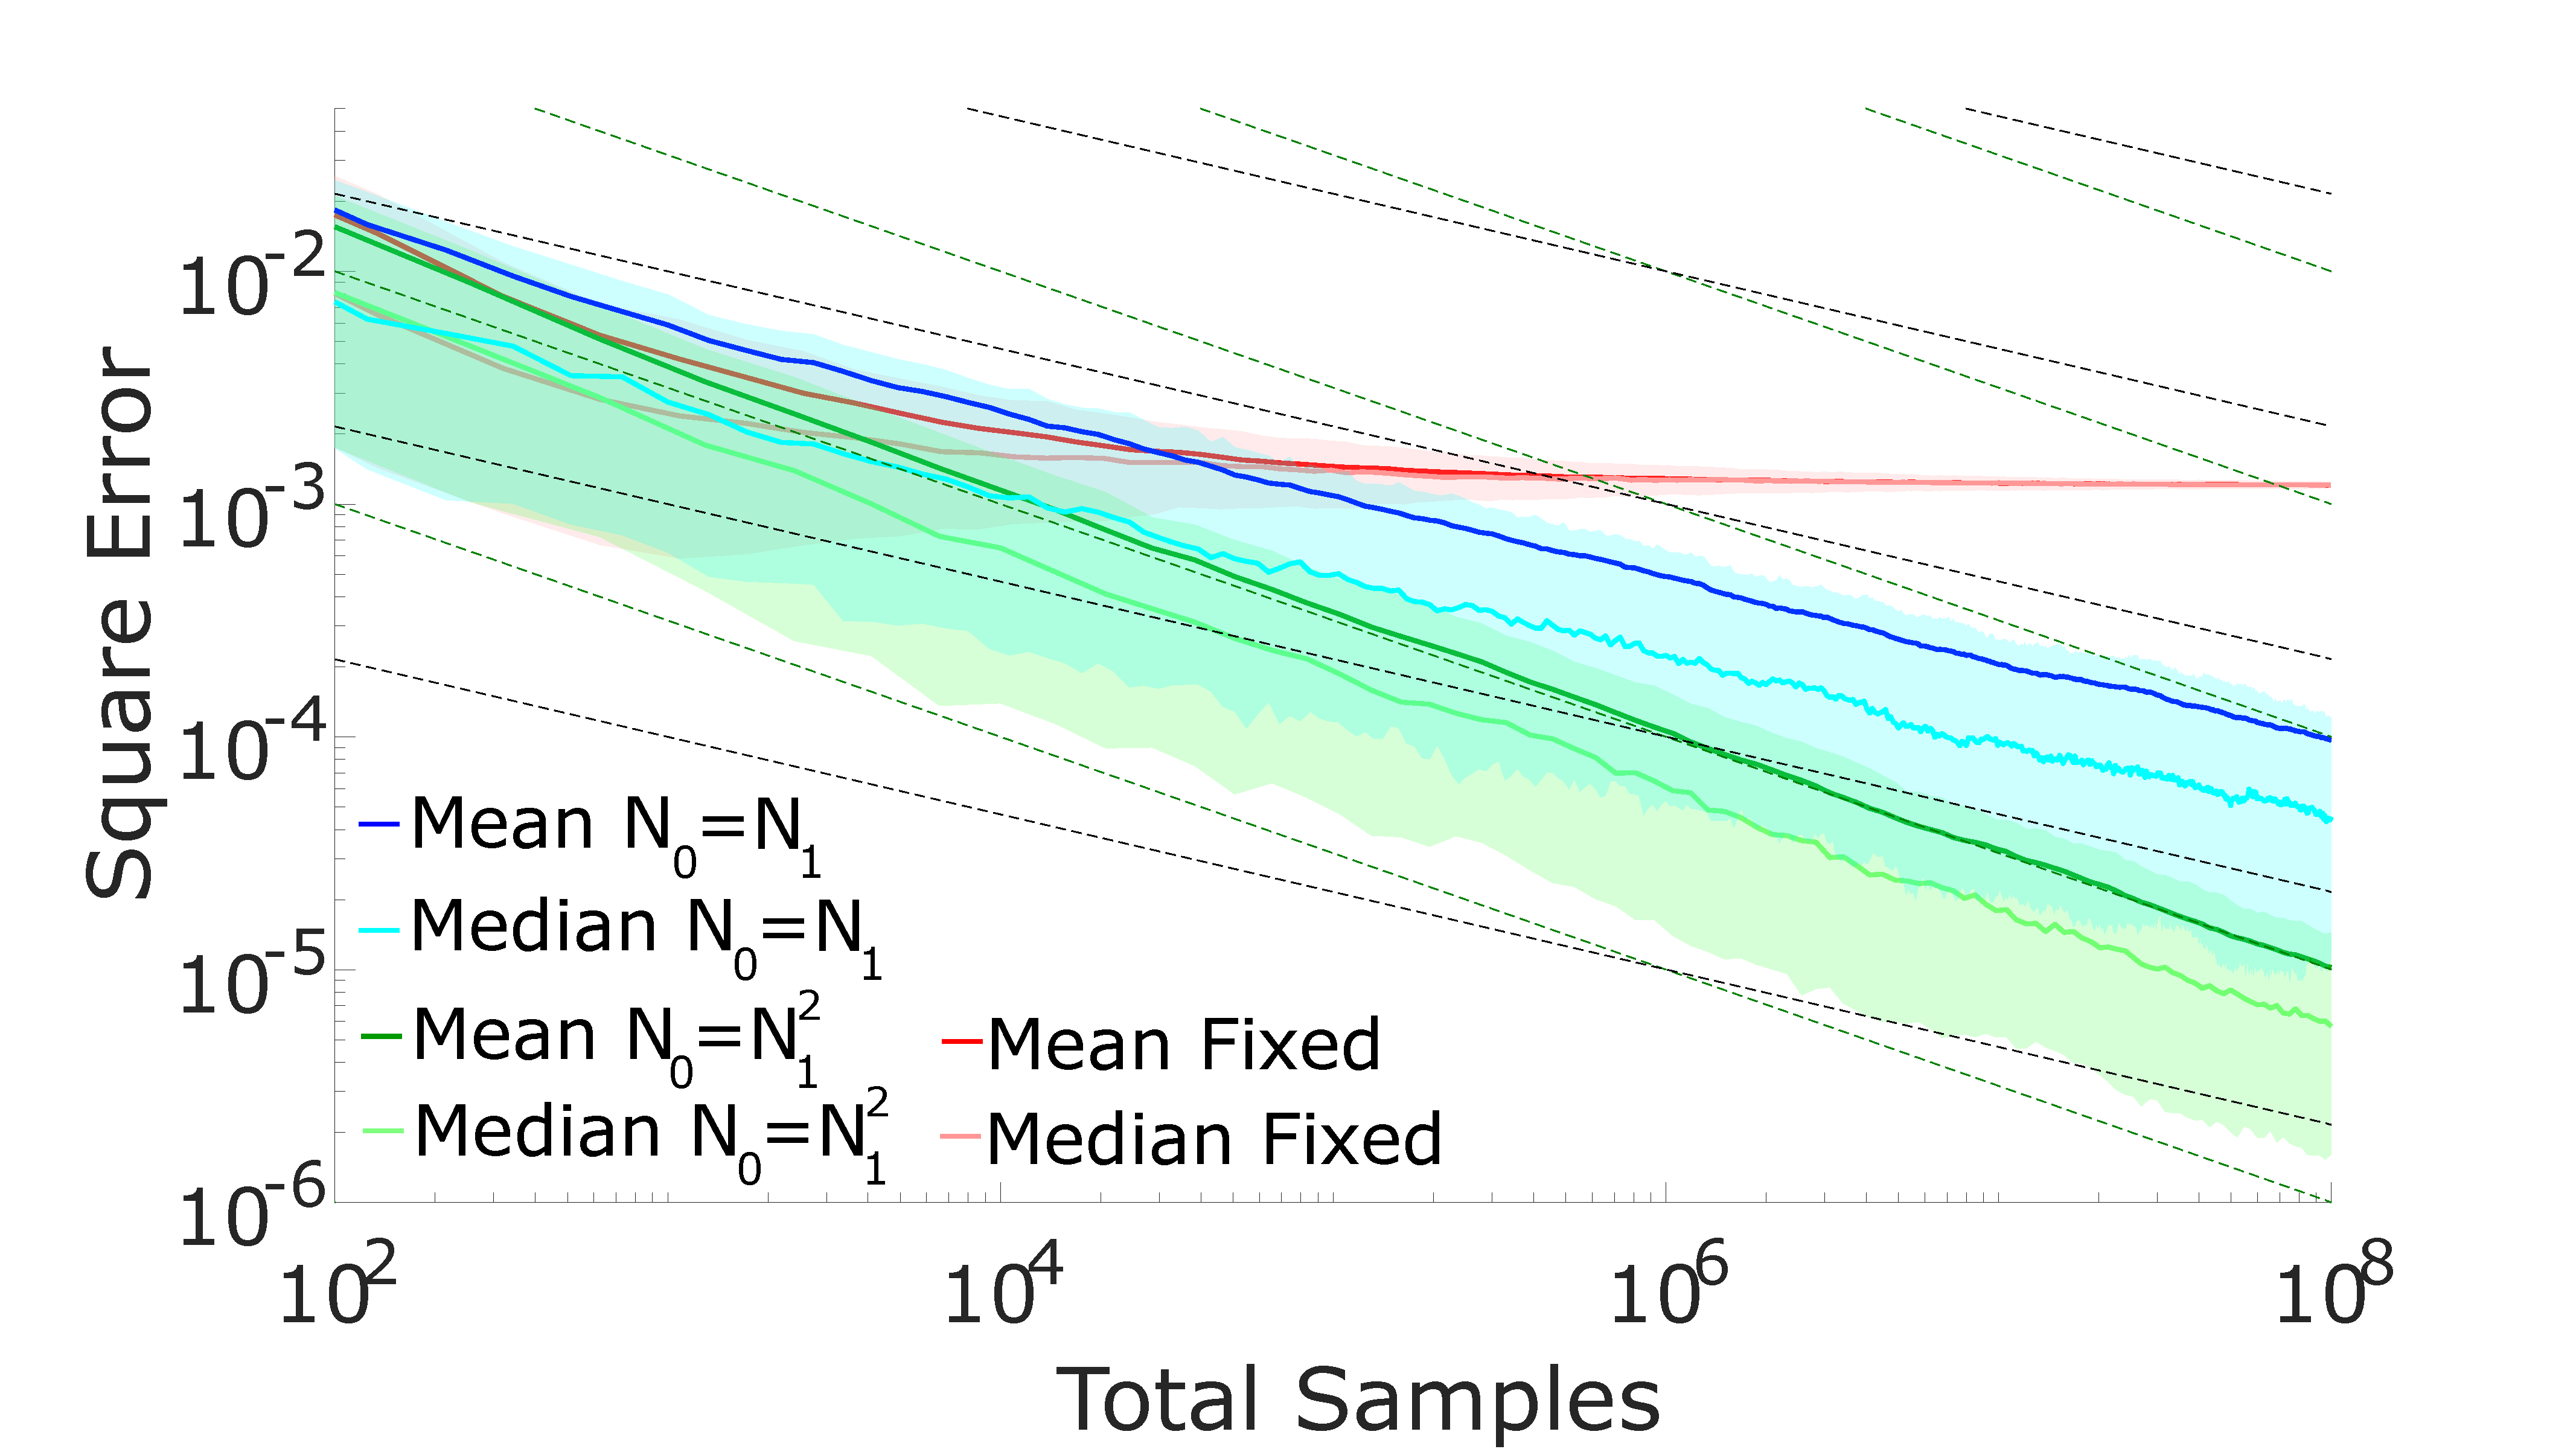
\includegraphics[width=0.5\textwidth,trim={1.5cm 0 3.5cm 0},clip]{repeat_nest_an}
	\caption{Empirical convergence of NMC to~\eqref{eq:repeat-nest} for an increasing total sample budget
		$T=N_0 N_1 N_2$.  Results are averaged over 1000 independent runs, while shaded regions give the 25\%-75\% quantiles.
		Shown in red is the convergence with a fixed $N_2=5$ and $N_1=N_2^2$, for which we see gives convergence
		to a biased solution, such that the error remains bounded as $T$ increases.  Shown in blue is the convergence
		when setting $N_0=N_1=N_2$, which we see converges at the expected $O(T^{-1/3})$ rate.  The black dashed lines
		provide a reference for this expected convergence of this estimator.  Shown in green is the convergence when
		setting $N_0=N_1^2=N_2^2$ which we see again gives the theoretical convergence rate, this time $O(T^{-1/2})$
		with the dashed green lines providing reference.\label{fig:multi-nest}}
\end{figure}	

We next consider the empirical performance of different strategies for choosing $N_0, N_1$, $N_2$ under a 
finite fixed budget $T=N_0N_1N_2$.
To do this, we define $\alpha_1$ and $\alpha_2$ such that $N_0 = T^{\alpha_1}$, 
$N_1 = T^{\alpha_2(1-\alpha_1)}$, and $N_2 = T^{(1-\alpha_1)(1-\alpha_2)}$ and then consider the variation in the
mean squared error with $(\alpha_1,\alpha_2)$.  In particular, we look to establish the optimal empirical
setting under the fixed budget $T=10^6$.  To investigate how sensitive the empirically optimal 
allocation is to the problem at hand, we consider both the model described in~\eqref{eq:repeat-nest} and 
also two slight variations.  The first keeps everything the same as~\eqref{eq:repeat-nest} except the following replacements
\begin{subequations}
	\label{eq:repeat-nest2}
	\begin{align}
		y^{(0)} &\sim \mathrm{Uniform}(-1,1), \\
		f_2 \left(y^{(0:2)}\right)&=\exp\left(\frac{y^{(1)}+y^{(2)}-y^{(0)}}{2}\right)
	\end{align}
\end{subequations}
while the second instead replaces $y^{(0)}$ with $y^{(0)}/10$ in the definitions of $f_1$ and $f_2$.  The two
respectively have analytic solutions of $I=11/32$ and $I=39/160$.

To 
try and find the optimal $(\alpha_1,\alpha_2)$ and establish the variation of the MSE more generally,
we ran a Bayesian optimization
algorithm (specifically the ``Black-box Bayesian optimization'' algorithm of~\cite{rainforth2015workshopbopp}) to
optimize the mean squared error, estimated by averaging $1000$ trials at each iteration, with respect to 
$(\alpha_1,\alpha_2)$.  This produced the performance characterizations shown in
Figure~\ref{fig:multi-tau}, corresponding to contour plots of $\log_{10} \left(\E \left[(I_0-\gamma_0)^2\right]\right)$ as
estimated by the surrogate function generated after $200$ Bayesian optimization iterations.
It further found respective optimal values for $(\alpha_1,\alpha_2)$ of  $(0.53,0.36)$, $(0.55,0.69)$, and $(0.38,0.45)$,
giving corresponding values for $(N_0,N_1,N_2)$
of $(1563,10,64)$, $(1957,73,7)$, and $(192,47,111)$.\footnote{Note that there is inevitably a small bias introduced
	by the fact that each $N_k$ has to be a whole number.  The true values of $T$ used for these solutions
	were $1000320,\; 1000027,$ and $1001664$ respectively.}  By comparison, the asymptotically optimal
setup suggested by our theoretical results is $\alpha_1=\alpha_2=0.5$ giving $N_0=977$, $N_1=32$, and 
$N_2=32$.
This demonstrates that even for relatively large values of $T$, the finite budget optimal allocation can vary significantly
from the asymptotically optimal solution.  We also see that the relative optimally can change quite significantly with
changes to the target problem.  For example, the second modification meant it was more preferable to run fewer iterations of
the outer estimator, perhaps because it reduced the relative importance of $y^{(0)}$ compared to the other variables
in $f_1$ and $f_2$.  However, further work is required to
establish concrete empirical guidelines and investigate whether methods that adaptively allocate the number of
samples might be feasible.  In the meantime, the asymptotically optimal choice (presuming continuous differentiability) 
of $N_0 \propto N_1^2 \propto \dots \propto N_D^2$ seems to a reasonable practical choice on average.

\begin{figure}[t]
	\centering
	\begin{subfigure}[b]{0.32\textwidth}
		\centering
		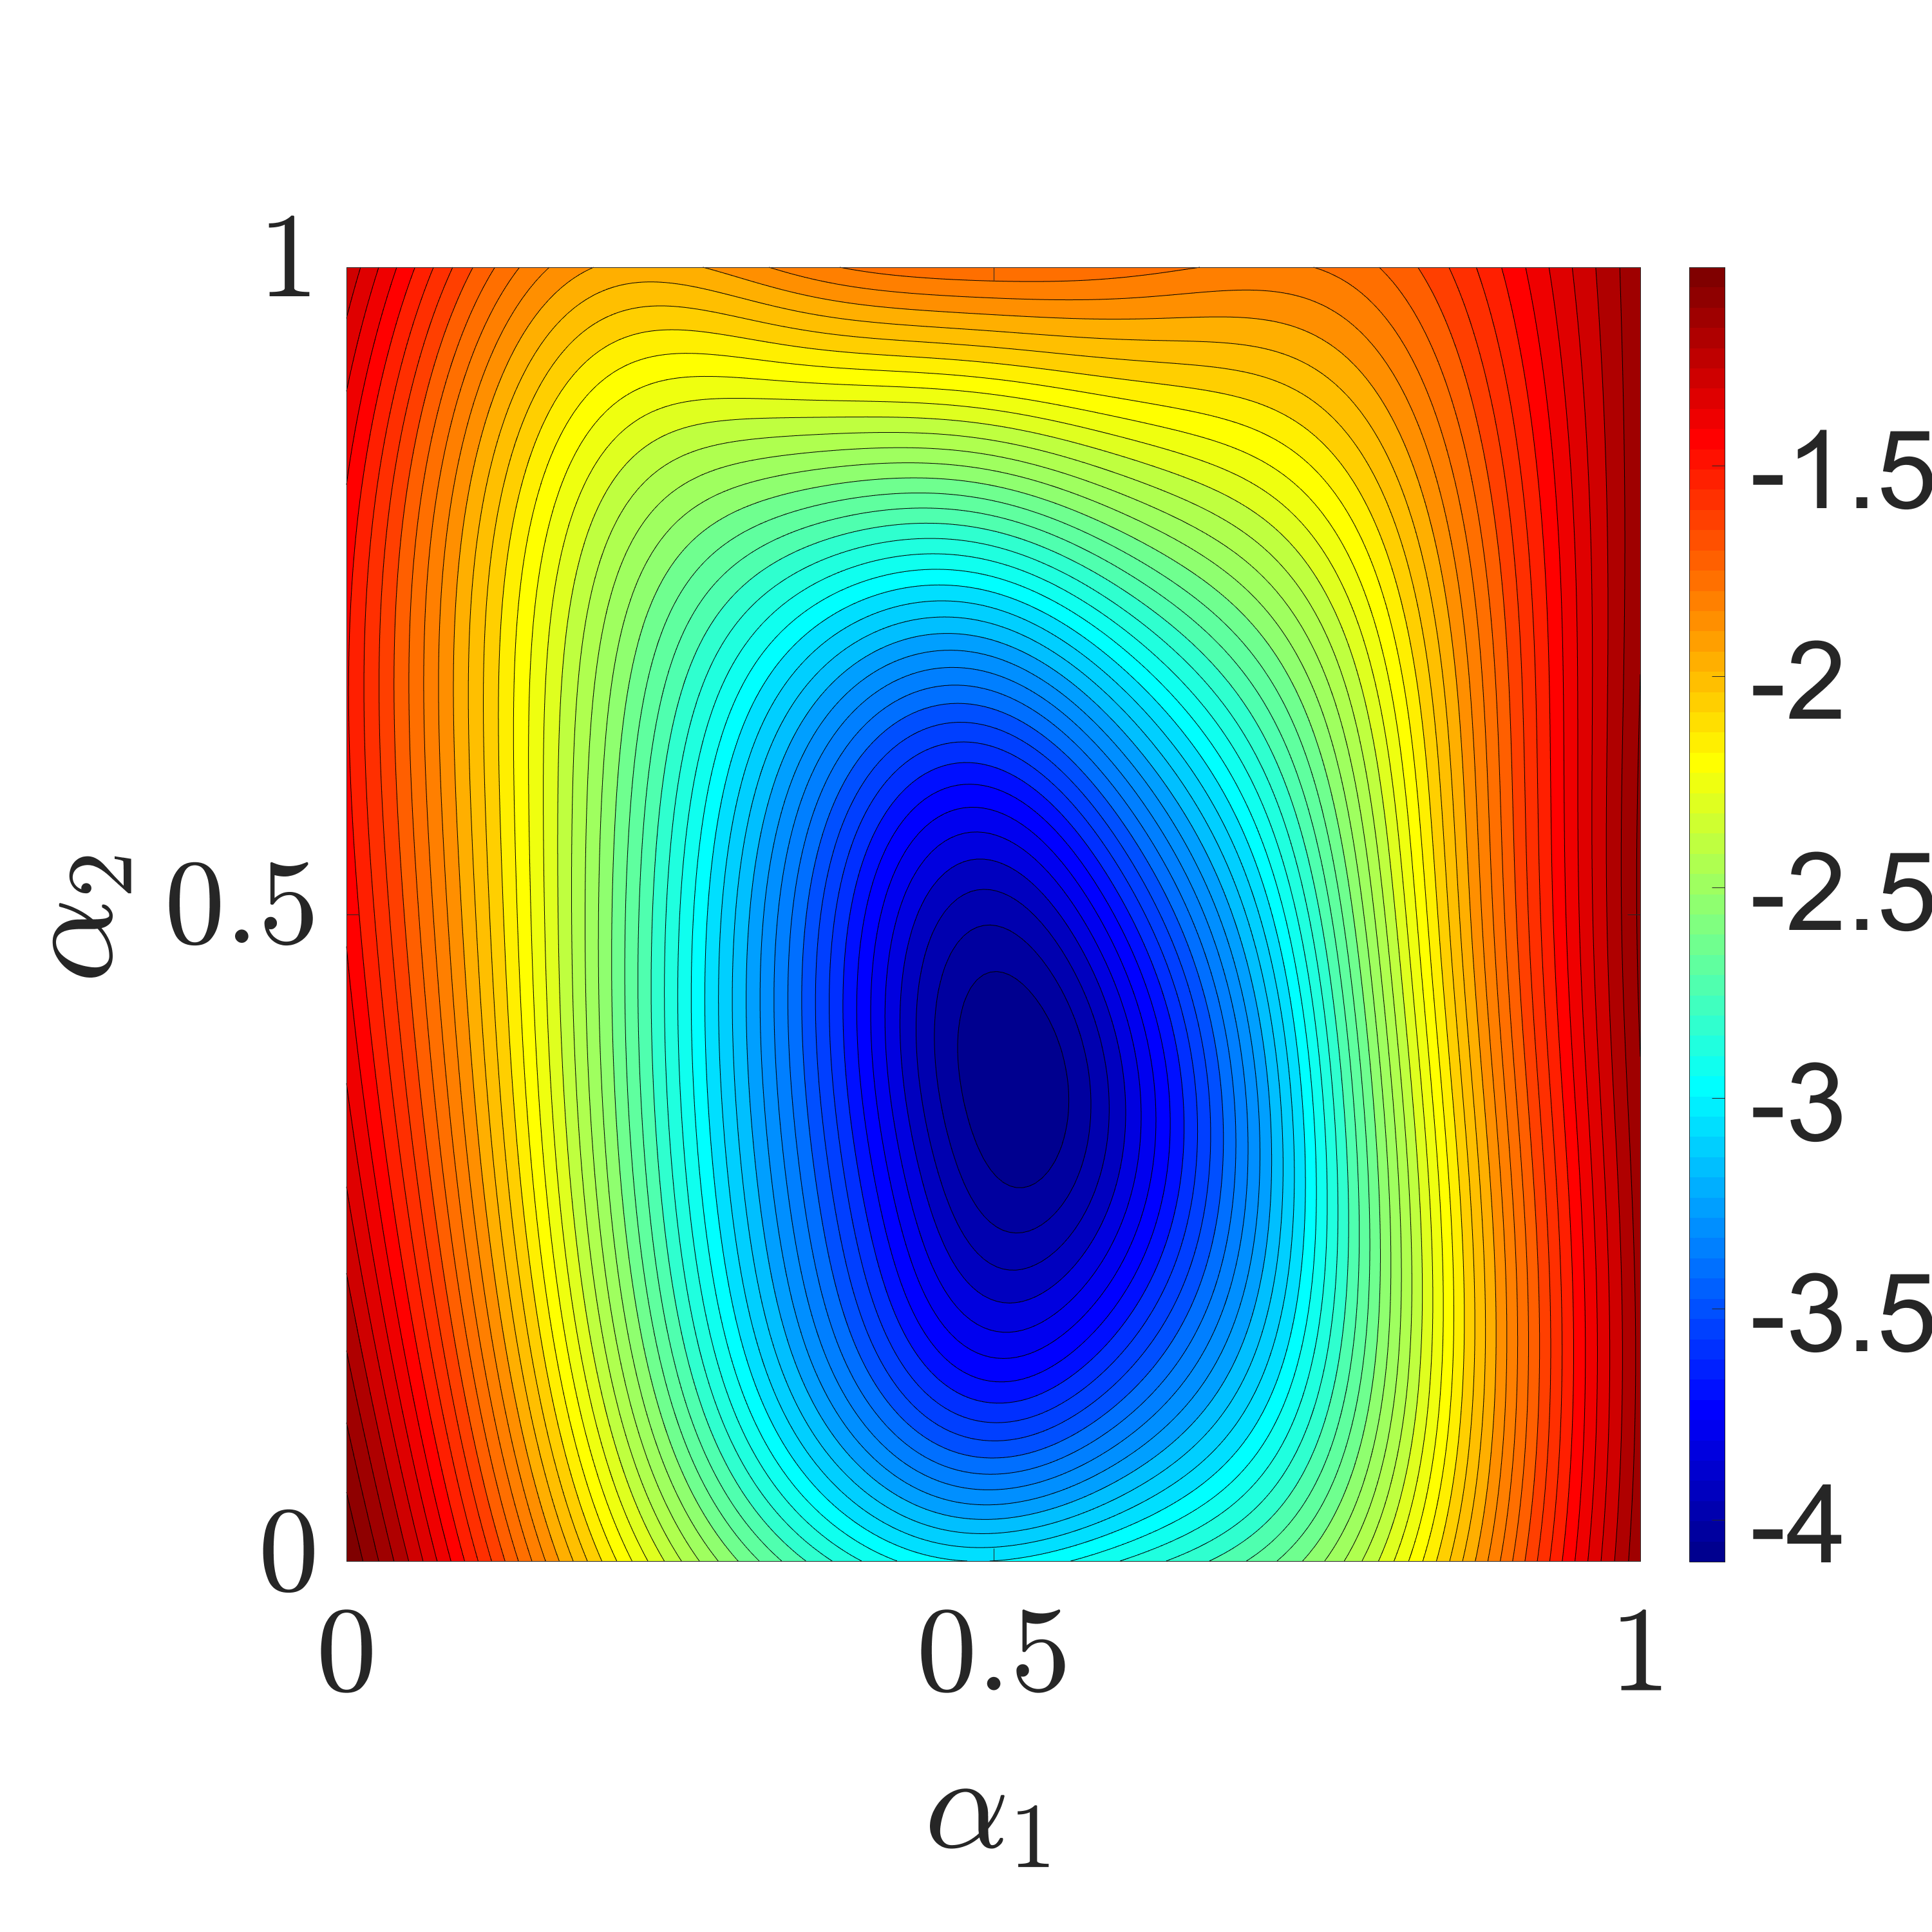
\includegraphics[height=0.88\textwidth]{tmax_1e6_model_3_contour_plot.pdf}
		\caption{Original}
	\end{subfigure}
	~\hspace{4pt}
	\begin{subfigure}[b]{0.32\textwidth}
		\centering
		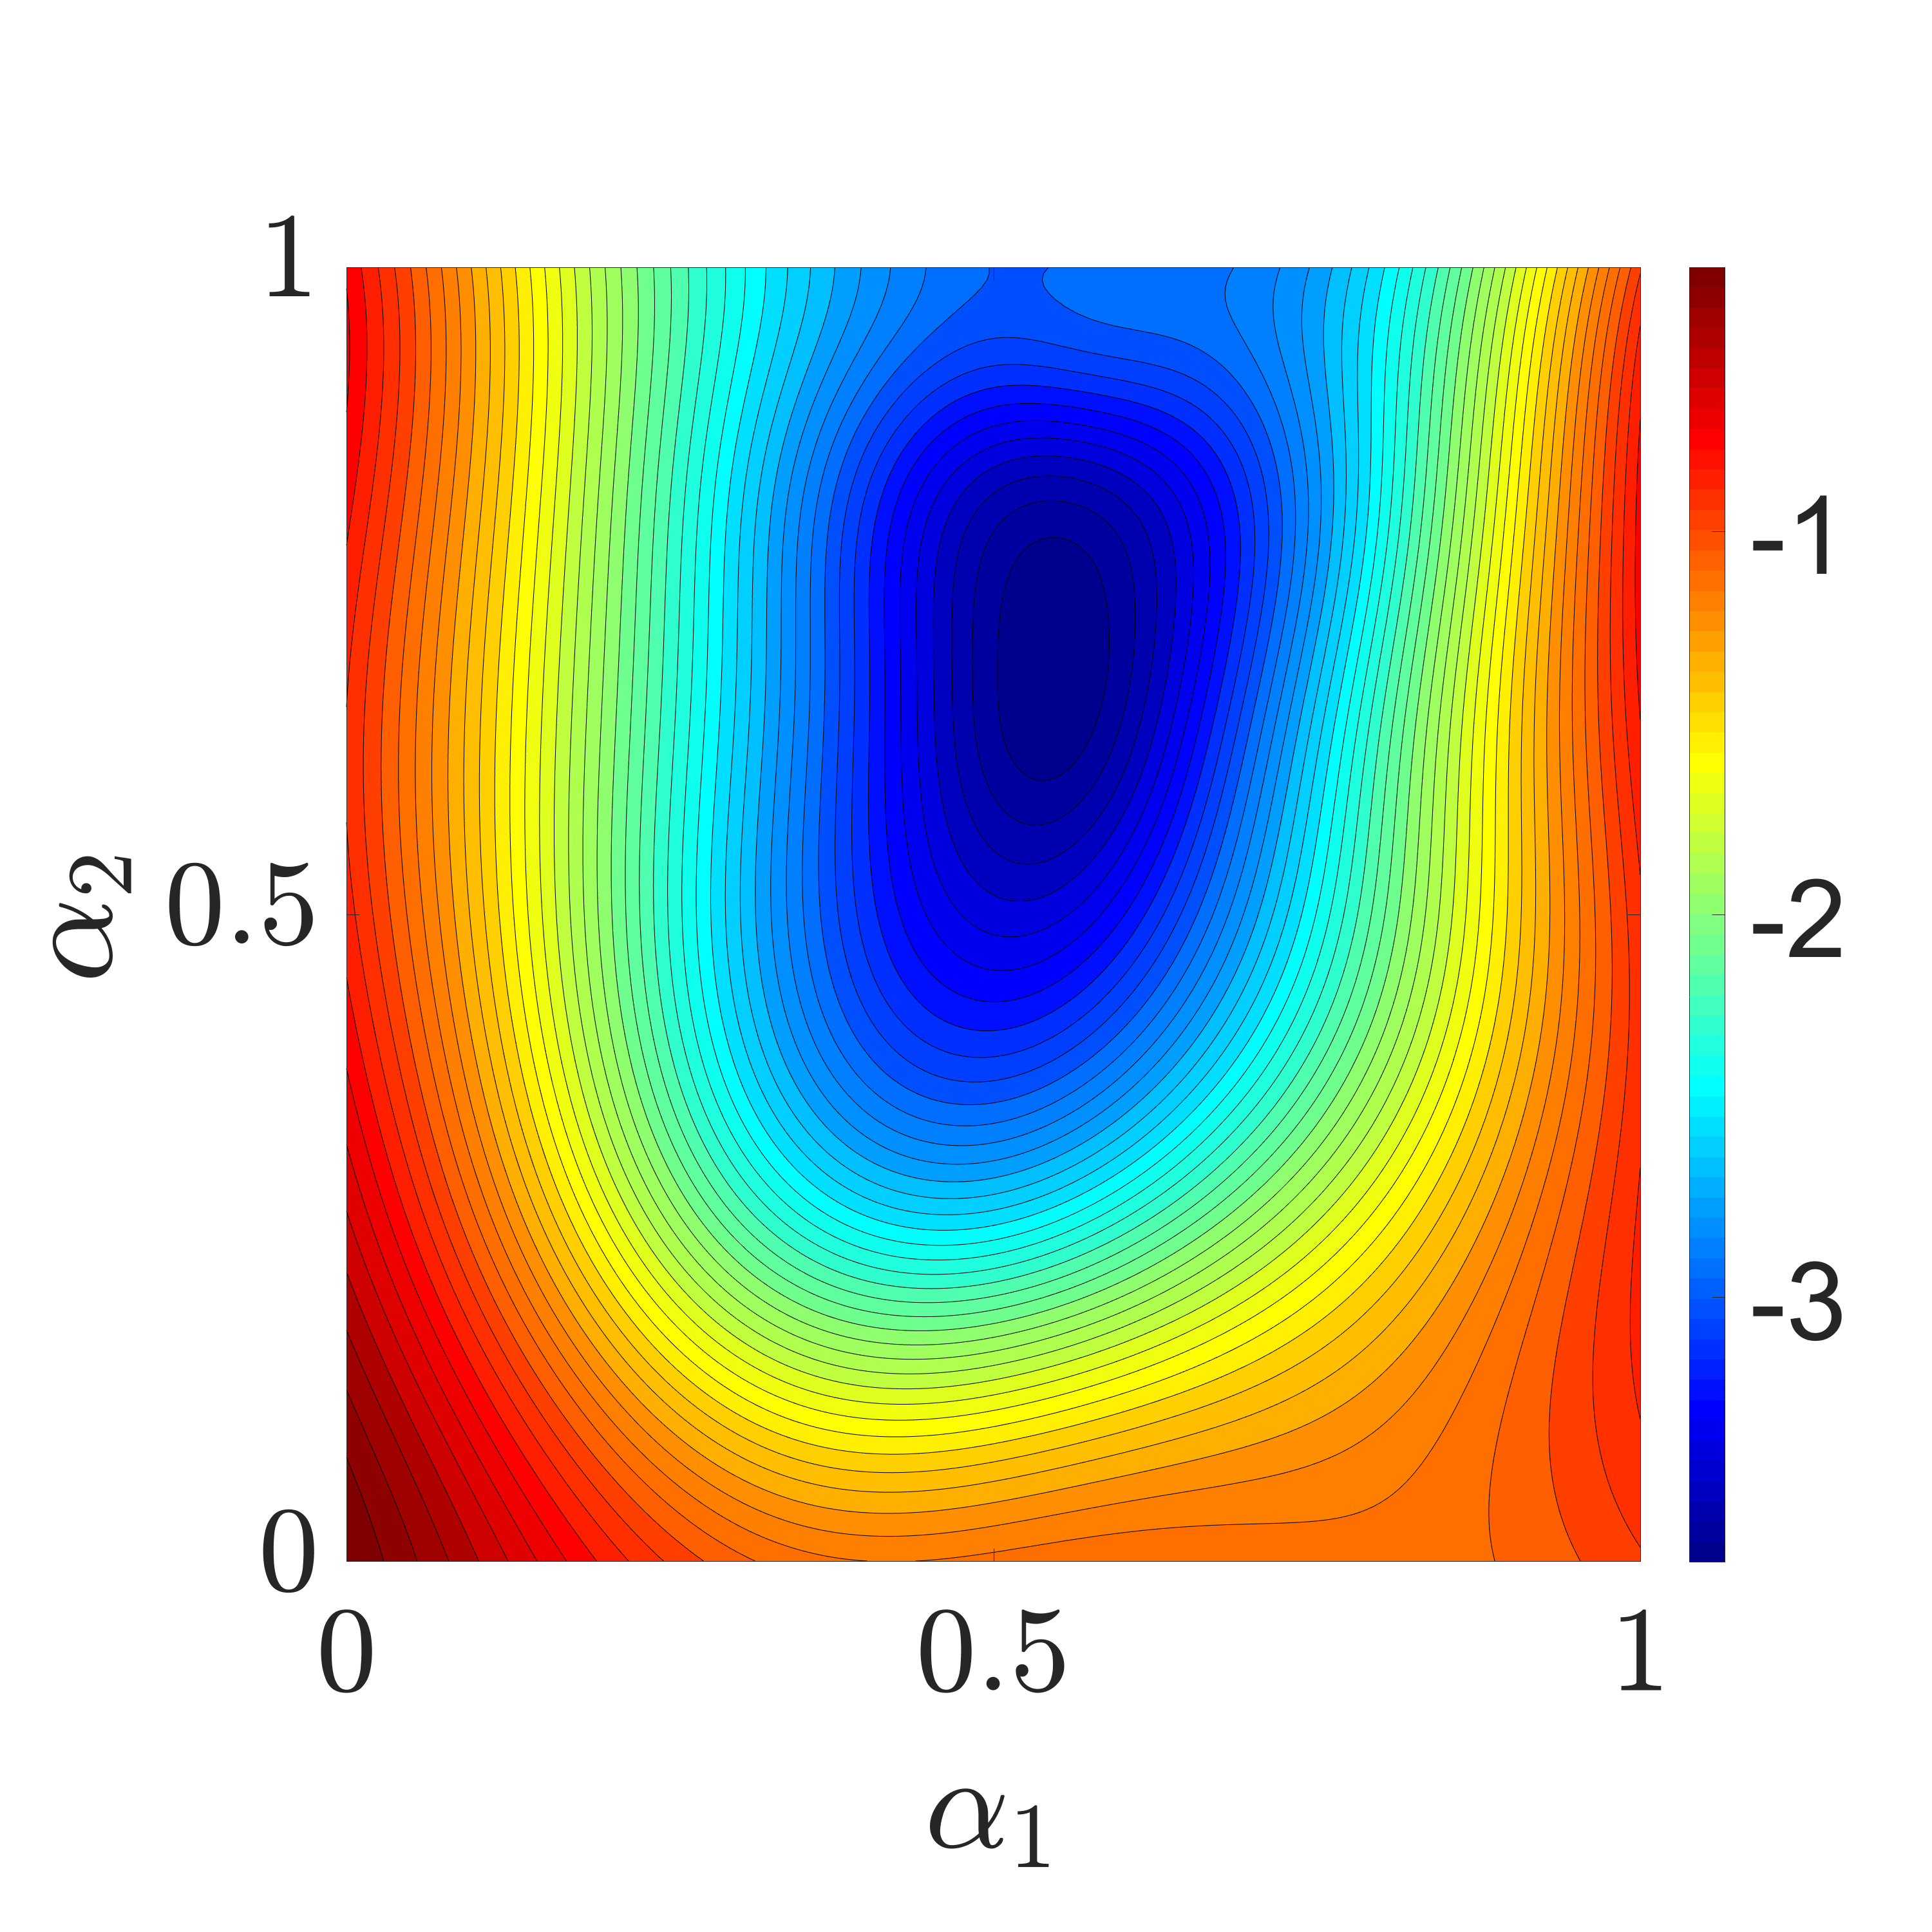
\includegraphics[height=0.88\textwidth]{tmax_1e6_model_2_contour_plot.pdf}
		\caption{First modification}
	\end{subfigure}
	~\hspace{-3pt}
	\begin{subfigure}[b]{0.32\textwidth}
		\centering
		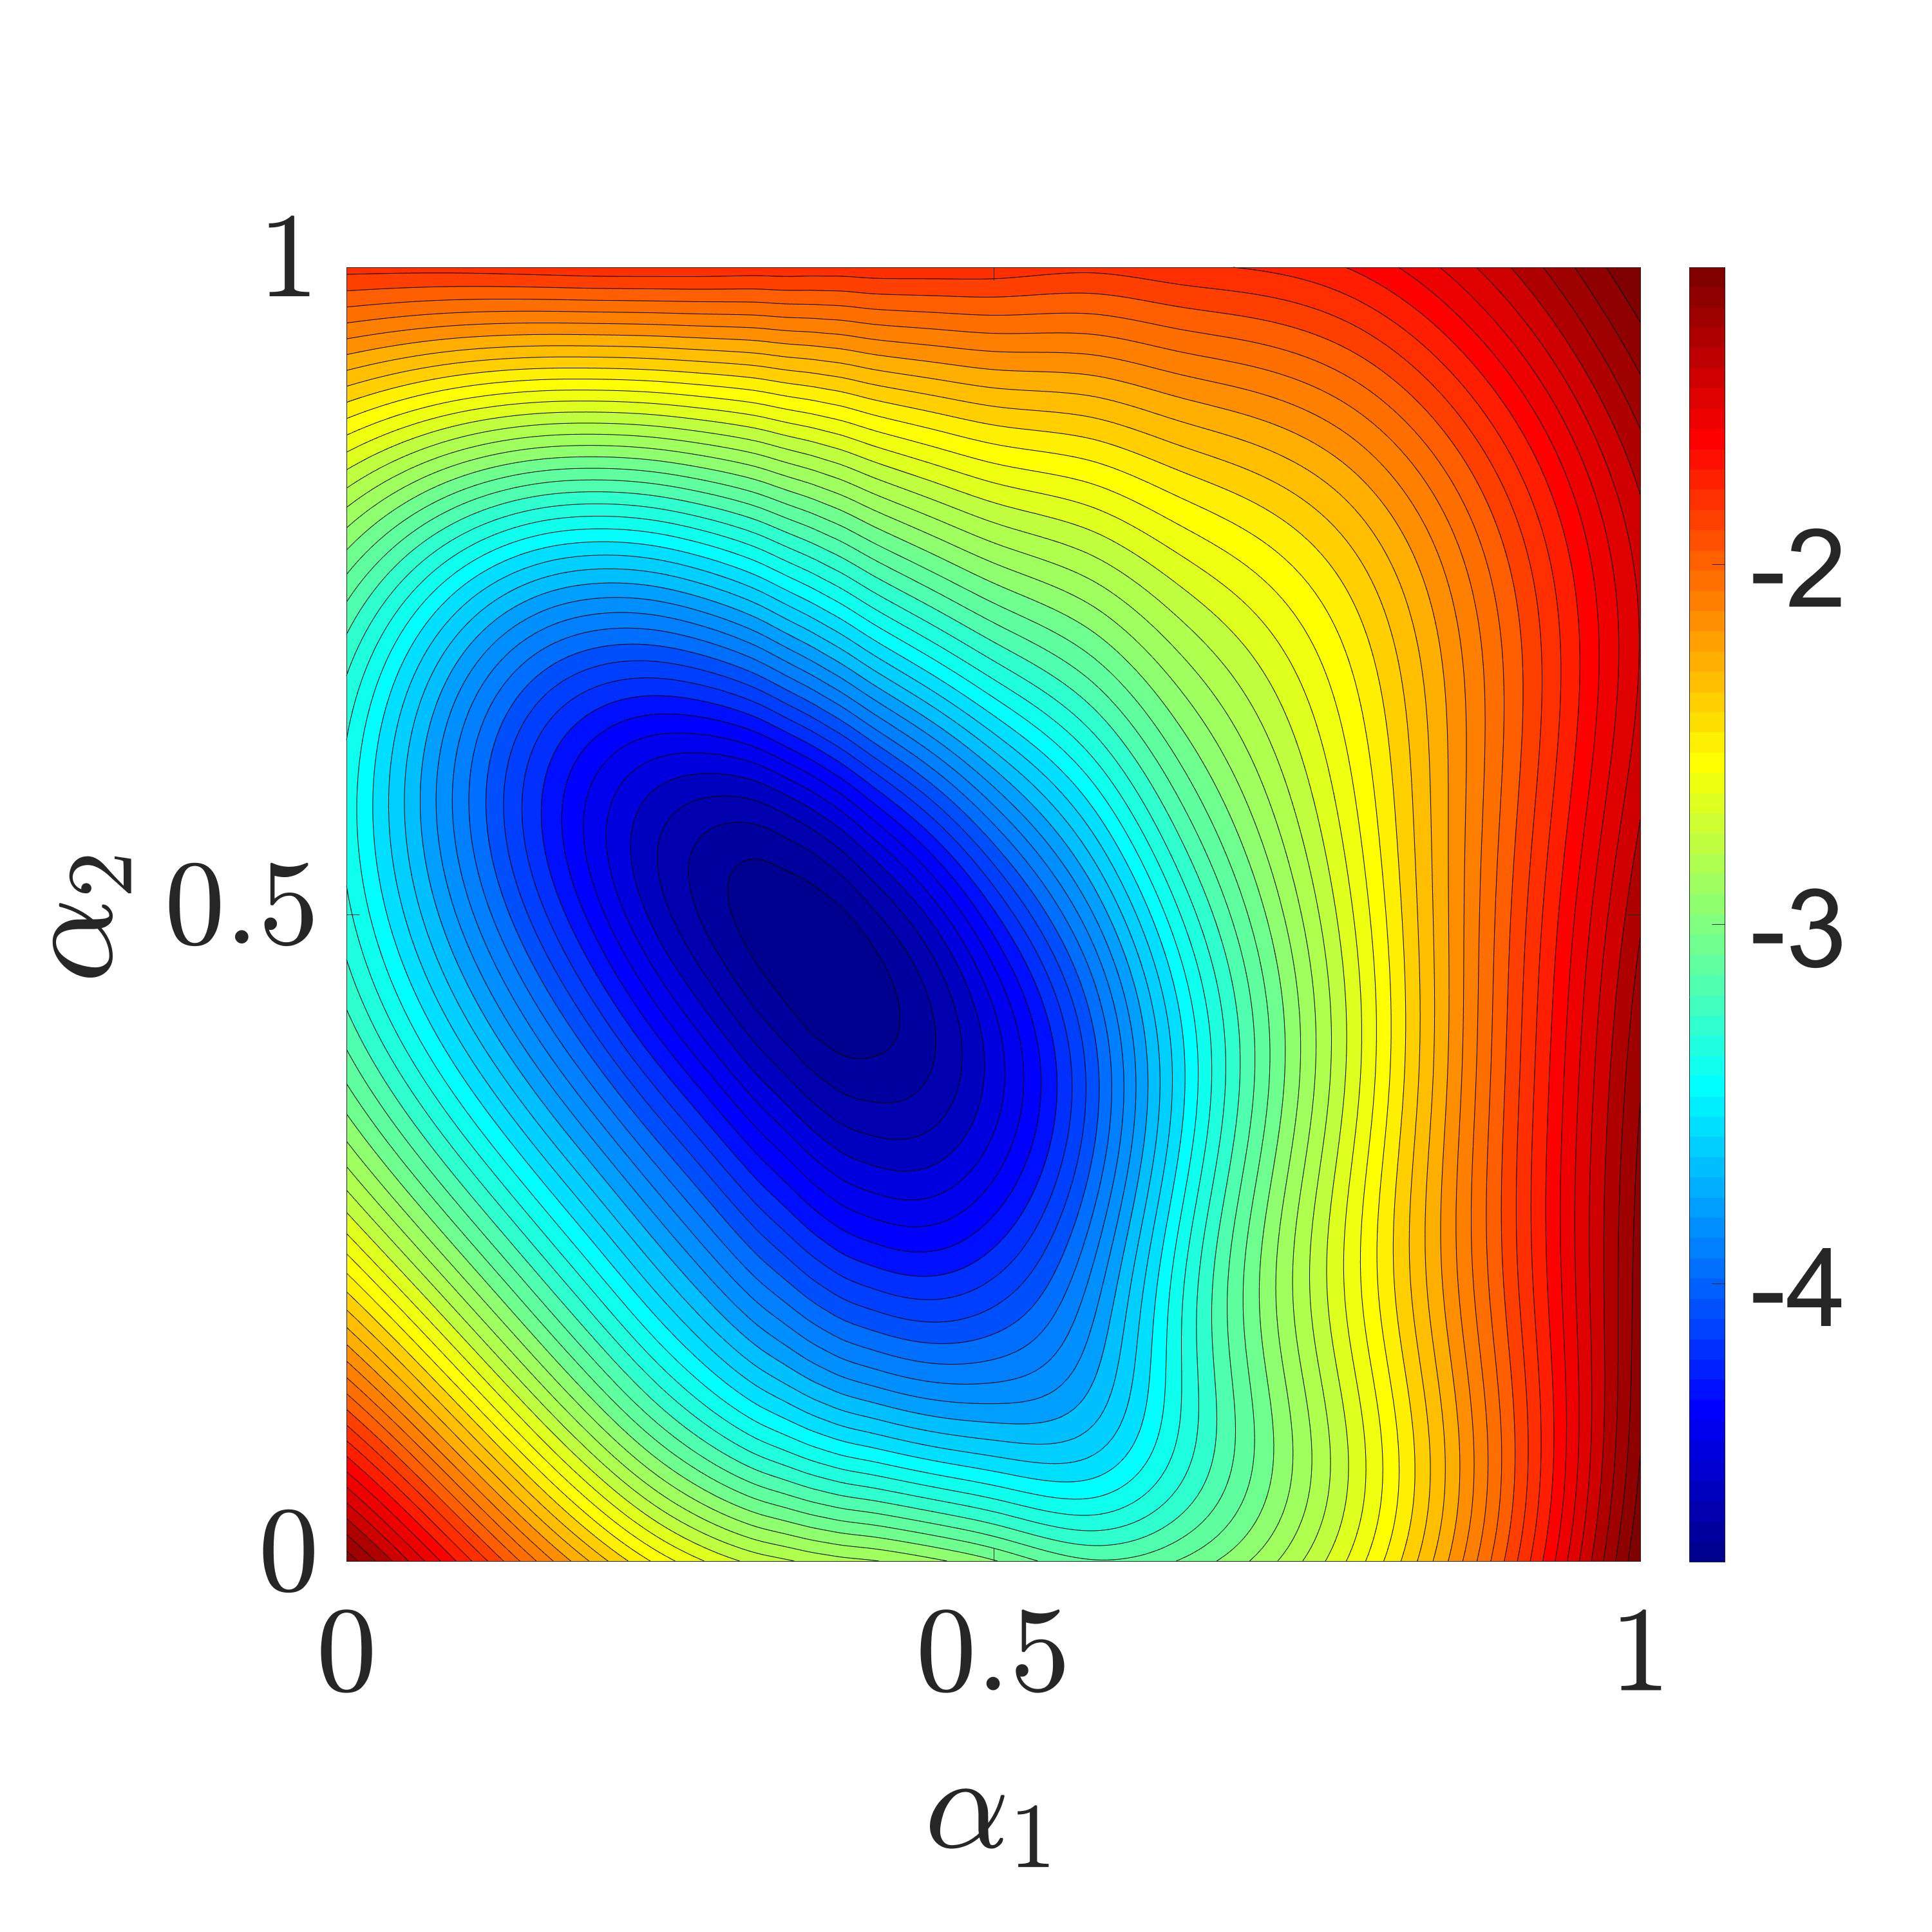
\includegraphics[height=0.88\textwidth]{tmax_1e6_model_4_contour_plot.pdf}
		\caption{Second modification}
	\end{subfigure}
	\caption{Contour plots of $\log_{10} \left(\E \left[(I_0-\gamma_0)^2\right]\right)$ (i.e. $\log_{10}$ MSE, estimated
		by averaging over $1000$ individual estimations)
		for different allocations of the sample budget $T=10^6$ between $N_0$, $N_1$,
		and $N_2$ for problem shown in~\eqref{eq:repeat-nest} and two modifications explained in
		the text.
		\label{fig:multi-tau}}
\end{figure}	